\documentclass[a4paper,11pt]{article}
\usepackage{geometry}
 \geometry{
 a4paper,
 total={210mm,297mm},
 left=1.25in,
 right=1.25in,
 top=1.25in,
 bottom=1.25in,
 }
\usepackage{graphicx}
\usepackage{amsmath}
\usepackage{amsfonts}
\usepackage{caption}
\usepackage{float}
\usepackage{subcaption}
\usepackage{breqn}
\usepackage{algorithm}
\usepackage{algorithmic}
%\usepackage[T1]{fontenc}
\usepackage{todonotes}
%\usepackage{graphicx}

\begin{document}

\title{Optimal Waterfilling Policy for Energy Efficient Wireless Networks}
\author{Sasank Chilamkurthy\\ Advisor: Prof. Abhay Karandikar}
\date{November 2014}
\maketitle

\begin{abstract}
We take up the power allocation problem for energy harvesting wireless networks. We restrict ourselves to waterfilling schemes because MDP formulation is complicated to solve. We give simulations and understand why there is a optimal policy. A simulation based optimization algorithm is proposed to determine the optimal policy.
\end{abstract}

\section{Intoduction}
We consider wireless communication using energy harvesting transmitters. Incremental recharge 
energy harvested from the environment will be available in random amounts as we cannot control environmental energy sources. In addition, wireless channel fluctuates randomly due to fading.
So, we need to design power allocation schemes which can adapt to both channel and energy recharge fluctuations.

We consider simplest system model with such a setting: single user transmission with a rechargeable battery. 
We assume that the recharge of the battery depends on current battery level. 
Optimal policy in a such a setting can be solved by modelling as an MDP. 
However state space is continuous and solving this online at the energy limited transmitter 
is impractical. So, we look at standard waterfilling scheme and give a simulation based  algorithm to chose the best waterlevel.

This report is organized as follows: First we describe the channel model and waterfilling scheme. 
Then we explain our energy harvesting transmitter node and simulate the system. Finally we propose an algorithm for determining optimal waterfilling policy.

\section{Wireless Channel Characterstics}
\subsection{Channel Model}
Wireless channel is characterized by the decay of signal strength due to various reasons like path loss, shadowing or Multi path fading. 
In multipath fading, which is our focus in this report, signals reach the receiver by two or more paths. 
Received component signals from these paths can interfere constructively or destructively. Destructive interference will result in fading of the signal. 
Moreover, due to relative motion between the transmitter and the receiver and/or movement of the reflecting objects, paths change randomly with time. 
This results in time varying amplitude and phase of the received signal.

This can be modelled as a time slot model in which channel fading characteristics do not change in a slot. This model is called Block Fading Channel. 
Under this model, if a transmitter transmits a signal $X_n$ in the slot $n$, then the received signal $Y_n$ is given by
\[Y_n = F_n X_n + Z_n \]

where $H_n$ corresponds to slot-varying gain due to multipath fading and $Z_n$ is complex Additive White Gaussian Noise (AWGN) with PSD $N_0$. 
$S_n = |F_n|^2$ is called channel state. Although a Markovian model for $F_n$ is possible, in this report we assume that $F_n$ is independent and identically distributed random variables.
Also, we only consider single user wireless channel.

\subsection{Waterfilling Policy}
Suppose we assume that transmitter has perfect knowledge of Channel State Information (CSI) and let $F_1,F_2 \dots F_M$ be a given realization of fading gains. We also assume that sufficient number of packets are always available for transmission at transmitter node.
If transmitter has an average power constraint $\bar{P}$, waterfilling policy gives  throughput optimal scheduling policy. This can be seen by solving following optimization problem:

\[ \max_{P1, \dots P_M} \frac{1}{M} \sum_{n=1}^M \log(1+ P_n |F_n|^2/N_0)\]

subject to 
\[\frac{1}{M} \sum_{n=1}^M P_n = \bar{P}\]

Observe that the objective function is average throughput over $M$ slots and the constraint corresponds to average power constraint.
This problem can be solved using standard Lagrangian relaxation and a solution can be determined to be:
\[ P_n^* = \left (\nu - \frac{N_0}{|F_n|^2} \right )^+ \]

where $x^+$ denotes $\max(0,x)$ and $\nu$ satisfies 
\[ \frac{1}{M} \sum_{n=1}^M \left (\nu - \frac{N_0}{|F_n|^2} \right )^+ = \bar{P}\]

As $M \rightarrow \infty$, by ergodicity, this can be written as
\[ \mathbf{E} \left (\nu - \frac{N_0}{|F_n|^2} \right )^+ = \bar{P}\]
where the expectation is taken with respect to the stationary distribution of the channel states. Thus the optimal power allocation for slot with channel state $s$ can be expressed as  
\[ P_n^*(s) = \left (\nu - \frac{N_0}{s} \right )^+ \]

This policy is visualised in figure \ref{fig:water}. When channel is good, transmitter allocates more power and less power if channel is bad. 
If channel is worse than a certain limit, no power will be allocated at all.
This is very natural and this insight is used later.
This policy is called \emph{Waterfilling Policy} and parameter $\nu$ is called \emph{Water level}.


\begin{figure}
\centering
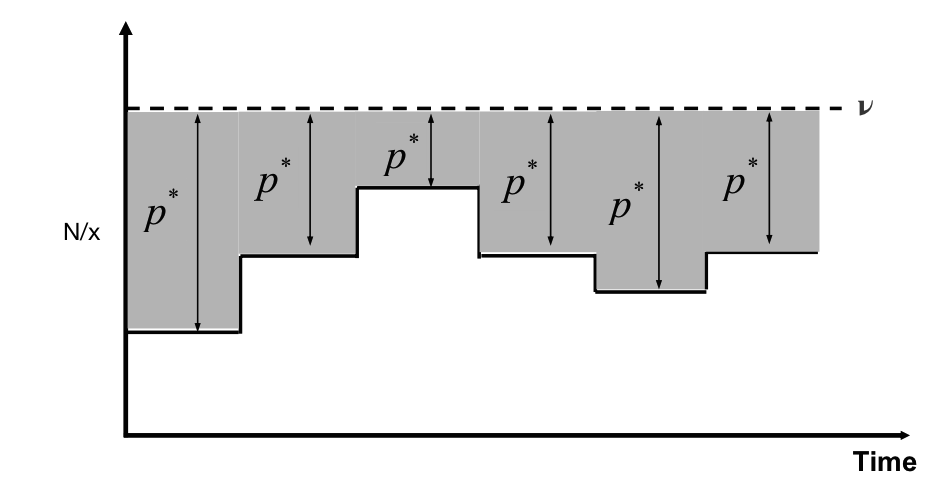
\includegraphics[width = 4in]{waterfilling.png}
\caption{Waterfilling Power Allocation}
\label{fig:water}
\end{figure}

\section{Energy Harvesting Transmitter}
In the preceding section, we assumed that transmthat as much energy as demanded by $P_n^*(s)$ is available with transmitter. However, if the transmitter relies on a battery for the energy then this may not be true. We now describe an energy harvesting transmitter.

We consider a transmitter node which has a rechargeable battery. The battery of the transmitter recharges using the energy harvested from the environment like solar energy, wind energy etc. The battery has a maximum capacity $E_{max}$.
Since we cannot control the amount of energy available from environment and it varies randomly
due to environmental fluctuations, we model the recharge as a random variable $K_i$.

Suppose in $i$th slot, $E_i$ is energy available in the battery, $P_i$ is energy consumed for transmission, then the energy available in the battery in $i+1$ th slot is given by:
\begin{equation}
 E_{i+1} = \min(E_i - P_i + K_i,E_{max}) 
\label{eq:battery}
\end{equation}
Note that $P_i$ has to be at most $E_i$. i.e. we cannot transmit more energy than what is available in the battery.

Random variable $K_i$ can be modelled in different ways. We can model it as a Markov chain or a iid random variables.
Another model can be that it depends on energy available in the battery in the current slot. 
\[K_i = U_i(1 - e^{\alpha(E_i - E_{max}) })\] 
where $U_i$ is a positive uniform random variable.
This model is more realistic because usually amount of the recharge to the battery decreases if battery is close to being full. Also, this allows us to modify equation \ref{eq:battery} as 
\begin{equation}
 E_{i+1} = E_i - P_i + K_i 
\label{eq:bettery}
\end{equation}
Because $P_i \geq 0$ and $K_i = 0$ if $E_i = E_{max}$, $E_{i+1}$ cannot
be more than $E_{max}$.
We consider this model in this report

As before we assume that transmitter has access to full channel state information and sufficient number of data packets are always available for transmission. 


\subsection{Optimal Policy} 
Our aim is to find optimal power allocation for the above system to maximise throughput. Observe that $E_{i+1}$ depends only on $E_i$ and therefore $E_i , i \geq 1$ is a Markov chain. 
This immediately leads us to formulate this system as an MDP.

Markov Decision Process is has 4 necessary components: state space, decision space, state evolution and reward function. Techniques of value iteration and policy iteration can be used to find decisions to maximize total expected reward.

In our system, state can be denoted by pair $(E_i,F_i)$ i.e energy available in the battery and fading state in the $i$th slot. 
So, state space is $[0,E_{max}] \times \mathbb{R}$. 
Decision process is power transmitted in $i$th slot, $P_i \in [0,E_i]$ and therefore 
decision space is $[0, E_i]$.
State evolution is given by equation \ref{eq:battery}. Reward for decision $P_i$ when system is in state $(E_i,F_i)$ is given by $R_i(E_i,F_i,P_i) = \log(1+ P_i |F_i|^2/N_0)$.
Our objective is to maximise 
\[ \bar{R} = \frac{1}{M} \sum_{i=1}^M \mathbf{E} [R_i(E_i,F_i,P_i)] = 
\frac{1}{M}\sum_{i=1}^M\mathbf{E} [\log(1+ P_i |F_i|^2/N_0)]\] 

Such a throughput Optimal policy can be found using policy or value iteration on this MDP. However, these iterations is impractical to be implemented on a battery powered transmitter node as state space is continuous. 
Therefore, we restrict search space to certain policy schemes. Excellent heuristics of water filling policy described in the previous section makes it a natural candidate. 
However energy demanded for transmission by water filling policy corresponding to water level parameter $\nu$, \[ P^\nu_i = \left (\nu - \frac{N_0}{|F_i|^2} \right )^+\] 
can be more than the energy actually available for the transmission in the battery, $E_i$. So, we need to modify water filling scheme. We have two possible choices for such modification
\begin{description}
\item[Choice 1]: If $P^\nu_i > E_n$, then $P_i = 0$ and $R_i(E_i,F_i,P_i) = 0$\\
If water filling scheme demands more energy than is in the battery, we transmit nothing and wait for next slot.

\item[Choice 2]: If $P^\nu_i > E_n$, then $P_i = E_i$ and $R_i(E_i,F_i,P_i) = \log(1+ E_i |F_i|^2/N_0)$\\ 
If the channel is so good that $P^\nu_i > E_n$, then we transmit using whatever energy we have available in the battery.
\end{description}
It is not a good idea to wait for transmission for next state when the current channel state is good as in choice 1. It is rather profitable to transmit using whatever energy is available in the battery. So, we follow choice 2.

This modifies water filling policy as following: 
\[P_i^\nu(E_i,F_i) = \min\left(E_{i},\left (\nu - \frac{N_0}{|F_i|^2} \right )^+\right)\] 


Since we are restricting to such modified water filling schemes, we only need to optimize water level parameter $\nu$ of the water filling policy to maximize average expected throughput
\[ \bar{R}(\nu) =  \frac{1}{M}\sum_{i=1}^M\mathbf{E} [\log(1+ P_i^\nu |F_i|^2/N_0)]\] 

We will simulate the system to understand the structure of $\bar{R}(\nu)$.

\section{Simulations}
For each water level $\nu$, we simulate $M$ slots. We generate a sample path 
of the system are generated and average throughput is calculated.
We generate $t$ such sample paths and mean of average throughputs for the $t$ sample paths will be an approximation the expected average throughput $\bar{R}(\nu)$.

%Independent and indentical Rayleigh distribution is assumed for channel states and battery is assumed to start from full charge.

Figure \ref{fig:path} shows a sample path of the system when $\nu = 0.45$. Figure 
\ref{fig:througput} plots $\bar{R}$ as a function of $\nu$. 
Figure \ref{fig:power} displays power quantities involved for each $\nu$.



\begin{figure}[H]
\centering
\includegraphics [width=3.5in]{{WaterLevel=0.45-p2}.eps}
\caption[fig:path]{A slice of sample path for \texttt{waterlevel} ($\nu$) = 0.45}
\end{figure}

\begin{figure}[h]
\centering
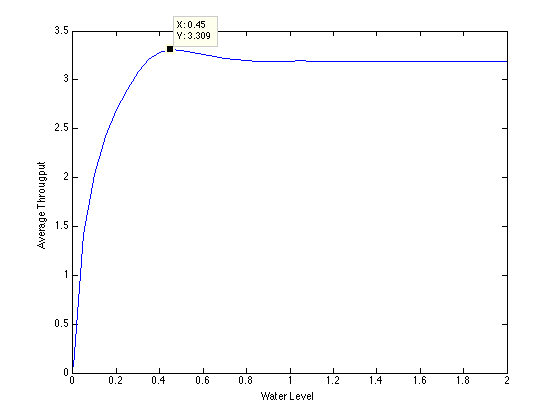
\includegraphics [width=3.5in]{AverageSimulation_02.png}
\caption[fig:througput]{Expected average throughput $\bar{R}$ vs. \texttt{waterlevel} ($\nu$)}
\end{figure}

\begin{figure}[h]
\centering
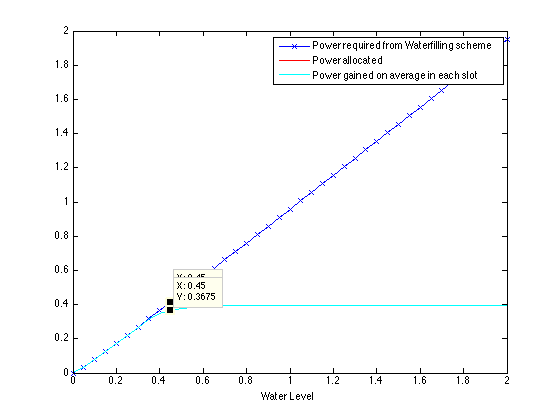
\includegraphics [width=4in]{AverageSimulation_01.png}
\caption{Expected power values of different quantities vs. \texttt{waterlevel} ($\nu$)}
\label{fig:power}
\end{figure}


Figure \ref{fig:path} suggests that $\bar{R}(\nu)$ saturates for large $\nu$. 
This is clear because if $\nu$ is large, unmodified waterfilling scheme always demands more energy than what is in battery. 
In particular, if $\nu\geq E_{max} + \frac{N_0}{|F_{min}|^2}$ then $\forall i \in N$
\[ \nu - \frac{N_0}{|F_i|^2} \geq  E_{max} + \frac{N_0}{|F_{min}|^2} - \frac{N_0}{|F_i|^2} \geq E_{max} \geq E_i\]
thus, 
\[P_i^\nu(E_i,F_i) = \min\left(E_{i},\left (\nu - \frac{N_0}{|F_i|^2} \right )^+\right)
 = E_i
\] 
therefore, we are transmitting all the energy that is available in the battery for all slots. From equation \ref{eq:bettery}, $E_{i+1} = K_i$. 
\begin{align*}
\bar{R}(\nu) &=  \frac{1}{M}\sum_{i=1}^M\mathbf{E} [\log(1+ P_i^\nu |F_i|^2/N_0)] \\
&= \frac{1}{M}\sum_{i=1}^M\mathbf{E} [\log(1+ K_{i-1}|F_i|^2/N_0)] \\
\end{align*}
Therefore $\bar{R}(\nu)$is independent of $\nu$. This also explains the saturation of power allocated, $\mathbf{E}[\sum_{i=1}^MP_i/M]$ in the figure \ref{fig:power}

For the $\nu \geq E_{max} + \frac{N_0}{|F_{min}|^2}$, we are forgoing the advantage of having battery to save up energy for future good states and greedily transmitting all the energy
gained from recharging. So, clearly these $\nu$ do not represent the optimal waterlevel parameter

\medskip

If $\nu \leq \frac{N_0}{|F_{max}|^2}$, then $\forall i \in N$
\[ \nu - \frac{N_0}{|F_i|^2} \leq \frac{N_0}{|F_{max}|^2}- \frac{N_0}{|F_i|^2}  \leq 0
\] 
Therefore,
\[P_i^\nu(E_i,F_i) = \min\left(E_{i},\left (\nu - \frac{N_0}{|F_i|^2} \right )^+\right)
 = 0
\] 
and 
\[ \bar{R}(\nu) = 0 \]

Thus we can restrict our search for $\nu$ to the region $\left [\frac{N_0}{|F_{min}|^2},E_{max} + \frac{N_0}{|F_{min}|^2}\right ]$.
For large $\nu$, we will be draining the battery and we will not save up for future good channel slots. On the other hand for small $\nu$, we will not be spending as much energy as we can and we will not be able to tap all the recharge from the energy harvesting.
Thus, there exists a $\nu$ in between which achieves a balance between saving and recharging and maximizes the throughput.


\section{Simulation Based Optimization of $\bar{R}(\nu)$}
Expected average throughput is a function of the entire system which in turn depends on choice 
of the parameter $\nu$. In particular, for a given water filling policy, state of the system $(E_n,F_n)$ is a Markov chain whose transition probabilities depend on the waterlevel parameter $\nu$ and the reward function is 
\[ \bar{R}(\nu) =  \frac{1}{M}\sum_{i=1}^M\mathbf{E} [\log(1+ P_i^\nu(E_i,F_i).|F_i|^2/N_0)]\] 

Since direct evaluation of these transition probabilities  and the derivative of $\bar{R}(\nu)$ is impractical, we resort to simulation based optimization.

For small $\delta_n$, we generate independent sample paths using simulation 
\[(\hat{E}_1, \hat{F}_1) ,(\hat{E}_2,\hat{F}_2), \dots, (\hat{E}_M,\hat{F}_M)\]
corresponding to $\nu = \nu(n)+\delta_n/2$ and 
\[(\mathring{E}_1,\mathring{F}_2),(\mathring{E}_2,\mathring{F}_2),\dots, (\mathring{E}_M,\mathring{F}_M)\] 
corresponding to  $\nu = \nu(n) - \delta_n/2$
and perform the iterate 
\begin{dmath}
\nu(n+1) = \nu(n) + a(n)
\left(\frac{\sum_{i=1}^M \log(1+ P_i^{\nu+\delta_n/2}(\hat{E_i},\hat{F_i}).|\hat{F_i}|^2/N_0) - \log(1+ P_i^{\nu-\delta_n/2}(\mathring{E_i},\mathring{F_i}).|\mathring{F_i}|^2/N_0)}{\delta_n} \right) 
\label{eq:iter}
\end{dmath}
Observe that the term in the brackets is an unbaised estimator for 
\[
\frac{\bar{R}(\nu + \delta_n/2) -  \bar{R}(\nu + \delta_n/2) }{\delta_n}
\]

Thus, equation \ref{eq:iter} can be rewritten as 

\begin{equation}
\nu(n+1) = \nu(n) + a(n)\left (\frac{\bar{R}(\nu + \delta_n/2) -  \bar{R}(\nu + \delta_n/2 ) }{\delta_n} + M(n) \right)
\end{equation}
for appropriately defined noise $M(n)$ whose expectation is 0. 
Thus this is a stochastic gradient scheme where gradient is estimated from simulations.
For numerical stability of the algorithm $t >1 $ sample paths can be used to estimate the gradient.

	\begin{algorithm}[H]
		\caption{OptimalWaterlevel}
		\label{algo:LearningGraph}
		\begin{algorithmic}[1]
			\STATE $\nu  = 0$
			\STATE $\Delta = \infty$
			\STATE $n = 1$
			\WHILE{$\Delta < \epsilon$}
			\STATE Simulate the system for $\nu + \delta(n)/2$
			\STATE Let $R_1 = $ average throughput
			\STATE Simulate the system for $\nu - \delta(n)/2$
			\STATE Let $R_2 = $ average throughput
			\STATE $\nu  = \nu + a(n)(R_1 - R_2)/\delta(n)$
			\STATE $\Delta = a(n)(R_1 - R_2)/\delta(n)$
			\STATE $n = n+1$
			\ENDWHILE
			\RETURN $\nu$
		\end{algorithmic}
	\end{algorithm}

If $a(n)$ and $\delta_n$ decrease sufficiently fast, this algorithm converges.
Experiments with this algorithm match with the optimal $\nu$ from figure 3.

\section{Conclusion and Future Work}
We have simulated the energy harvesting wireless networks under waterfilling schemes
and understood the evolution of the system.
A simulation based stochastic gradient scheme is proposed to optimize average expected throughput. 

Although experiments show that simulation based scheme converges, it will be of theoretical interest to prove that this actually converges under certain conditions. In particular, it will be interesting if it can be proven that average expected throughput $\bar{R}(\nu)$ is a quasi-concave function with respect to $\nu$ and there is a unique global maximum.



\begin{thebibliography}{4}

\bibitem{text2}
Abhay Karandikar and Nitin Salodkar, “Cross Layer Scheduling in Wireless Networks”,  in “Wireless Network Design: Optimization Models and Solutions Procedures”, Kennington, Jeffe; Olinick, El; Rajan, Dinesh (eds), Springer-Verlag, 2010

\bibitem{text} 
Cover, T. and Thomas, J. (1991). Elements of Information Theory, Wiley, New York.

\bibitem{paper1}
Vinod Sharma, Utpal Mukherji, Vinay Joseph and Shrey Gupta Optimal, Energy Management Policies for Energy Harvesting Sensor Nodes. IEEE Transactions on wireless communications, Vol. 9, No. 4, April 2010
\bibitem{dessert}
Vatsal Shah, Energy Efficient Scheduling Using Green Energy Sources, Dual Degree Dissertation, June, 2014, Indian Institute of Technology Bombay
\bibitem{paper2}
Omur Ozel, Kaya Tutuncuoglu, Jing Yang, Sennur Ulukus, Aylin Yener, Transmission with Energy Harvesting Nodes in Fading Wireless Channels: Optimal Policies, Ieee Journal On Selected Areas in Communications, Vol. 29, No. 8, September 2011
\end{thebibliography}


\end{document}
